%!TEX root = ../proposal.tex
\section{Proposed Method}
The aim of the research is explore the parameters of velocity, steering angle and velocity in autonomous cars to simulate critical crash scenario in crash report. The velocity and steering angle parameters are missing in the crash report. I have to identify the numerical values of velocity and steering angle that produce the collision of the vehicles. Secondly, relaxation on the structure assumptions of semi-structured and structured text to construct better natural language processing information extraction. \\

In short, the approach is to apply natural language processing and ontology techniques to extract key features from the semi-structured to unstructured text to create the configuration file. The configuration file contain the information to create the scenario in BeamNG and the dynamics, position of the car in crash scenario. The configuration file can be visualized on the Open Street Map to show the possible trajectory of autonomous vehicles. After the creation of scenario, the vehicle trajectory will be predicted to explore the velocity and steering angle parameter for the collision of vehicles. The number of simulations will be run to get the numerical values of the parameter of the critical crash scenario until the stop criterion is reached in the decision tree. On each simulation, the coordinates/path and the velocity will be extracted from the simulation to generate trajectory path, calculate the Structural Similarity Index Matching and Mean Square. The next numerical value of the parameter should be devise from the current simulation to reach the target point in the crash scenario. \\       

The procedure of automated test cases generation to explore the parameters of the car accident scenario is summarized in the Figure 2. \\

\subsection{Natural Language Processing}
In the growing world of internet and online services, the data is available in gigabytes in open source platforms and communicated in the form of text. The extracted text is available in the form of tabular data, unstructured data, and raw data in XML. Our target is to apply the Natural Processing algorithms to understand the human language that what are they saying about the environment and accident of autonomous cars.

\begin{figure}[H]
\centering
  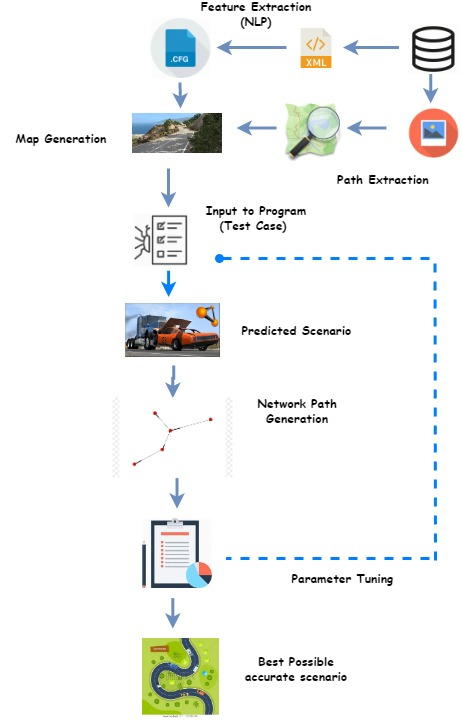
\includegraphics[scale=0.55]{pictures/Architecture_Diagram_Proposal_AT.jpg}
  \caption{Architecture Diagram}
\end{figure}

\subsubsection{Text Analysis and Features Extraction}
To generate the trajectory based on the car crash report, the following features need to be extracted using Natural language processing Algorithms. 

\begin{itemize}
  \item	Automotive Type
  \item	Weather conditions
  \item	Positions of the car relative to each other
  \item	Accident Type
  \item	Car behavior (Sequences)

\end{itemize}

All these features extraction is based on the information available in the semi-structured and unstructured data in the crash report. If the information is not available, the simulation will not be generated.

\subsubsection{Natural Language Processing Algorithm}
These individual steps are required to convert text into the machine-readable format for further processing.  The Natural language toolkit or Stanford language parse can be used to execute all the steps.

\paragraph{Tokenization Paragraph}
The initial step of analyzing the text content is to break down the paragraph into smaller sentences. Later, the sentences are break down into words to identify keywords, phrases, and symbols. 

\paragraph{Part of Speech Tagging}
Part of Speech tagging is useful for identifying the grammatical group of a given keyword based on the contextual information.  The word tags can be a Noun, Pronoun, Adjective, Verb, Adverb based on the preceding word and avoid disambiguation. 

\paragraph{Chunking (Shallow Parsing)}
Part of Speech tagging does not give enough information to retrieve the information about the sentence and waste time to parse the tree of the sentence. A shallow parsing is a technique that gives us a bunch of words related to our application-oriented processing such as Noun Phrase and Verb Phrase to get the semantic information. Alternatively, the subject, verb and object triples can be extracted from the sentences using stanford OpenIE. 

\paragraph{Dependency Tree Parsing}
In each sentence, there is a root words and all other words are directly or indirectly linked to root node. The dependency-based grammars is used to identify each word relationship with root node to get structural and semantic information about the sentence. The dependent words information help us to extract and generate the sequence of action describe in natural language. The Spacy,Penn Tree Bank and Stanford parser are the most useful libraries for dependency tree parsing. 

\paragraph{Co-reference resolution (anaphora resolution)}
In natural language, it is hard to identify the Pronouns,Noun Phrases and individual token/word with simple text mining techniques that point toward the same entity in the real world. Anaphora resolution find the right word that are connected mentioned entity in the sentence. 

\paragraph{Stops Word}
In sentence, there are unnecessary words/token that don't carry any meaning and does not determine and semantic relation between the words are called "Stops Word".The words like “the”, “a”, “on”, “is”, “all” are usually removed from the text to carry out further processing.  

\paragraph{Stemming and Lemmatization}
The aim of the stemming and lemmatization to reduce the word to base form considering the relationship of the words with each other. The stemming and lemmatization of the word make it easier to find the root of the entity of the word like environment, vehicle and road etc. These words will be further processing in entity recognition using Ontology.  
\subsubsection{Ontology-based Named Entity Recognition}
The ontology can be defined as the object that share the relationship with each other and belong to the same concept (category). Ontology is composed of Taxonomy, Relationship, Class Attributes and Rules/Axioms. As an example, putting the element "BMW" in category like animal/mineral/vehicle \cite{cucerzan2007large}. The element category will help us in determining the variables available for the reconstruction of crash scenario in self driving cars. \\

The other way of doing it is using the Named Entity recognition of Stanford parser but it is not applicable to our case because the domain of knowledge of Stanford parser is restricted to only 7 variables such as TIME, DATE, ORGANIZATION etc. The spaCy named entit  recognition will be applied to spread the domain of named entity recog\\

All thye information extracted is stored in the XML/JSON file, it will be further processed to create scenarios in Open Street Map and BeamNG. 

\subsection{NHSTA Trajectory Generation from Images - (Network Path Generation)}
The NHTSA crash viewer provide an information that how the car followed a path before the crash and after the crash. This information is usually displayed in the images. The manual user will interpret these images and create the original trajectory path of the vehicles. The original trajectory path will be compared with the predicted simulation path to to categorize the simulation and calculate mean square error with original NHTSA crash trajectory. The NetworkX \cite{SciPyProceedings_11} library enable us to convert the continuous data into discrete nodes.      

\begin{figure}[H]
\centering
  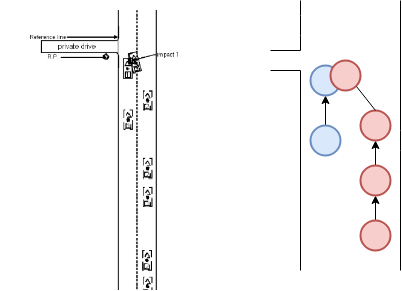
\includegraphics[scale= 0.4]{pictures/SO1_NET.png}
  \caption{Trajectory Network From NHTSA Image}
\end{figure}

\subsection{Open Street Map - (Optional)}
The Open Street Map (OSM) is an open source platform to extract the data about roads and nearby characteristic such as building in the given region of interest. Open Street Map allow users to edit map and use data free of cost. Our objective is to extract the data from the open street map according to the description given in the natural language processing. The roads can highways, urban road, rural road, junctions. However, the location is rarely specified in the description so we will assume our region of interest and try to extract the best possible scenario from Open Street Map. The car trajectory with different colors for each vehicle will be shown on the Open Street Map for visualizations. 

\begin{figure}[H]
\centering
  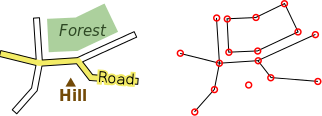
\includegraphics[scale= 0.7]{pictures/nodes-and-ways.png}
  \caption{Open Street Map Nodes}
\end{figure}

\subsubsection{Data Extraction from Open Street Map}
The Open Street Map\cite{haklay2008openstreetmap} data can be extracted from Xapi Api. After obtaining the response from API request, the XML object is parsed to extract the roads and link roads according to the tagged provided in the smart query. The target attribute is the width of the road and it can be filtered from large data-set and small visualization can be drawn on the Open Street Map. 

\subsection{Generation Test Cases Scenarios in BeamNG}
The BeamNG is open source tool for studying and developing vehicle accidents of self-driving cars with an integrated option of Artificial Intelligence. The BeamNG provide the realistic figures of car dynamics, car damage, environment and roads etc. It provides us the features to extract the data from the simulation, record videos for analysis and provide mechanism to set up speed, start, stop, steering angle, direction of car in the scenarios. Additionally, the BeamNG (3D) will be used to simulate the scenario demonstrated in Open Street Map (2D) with an access to unlimited research version of BeamNG.  
 
\subsubsection{Environment Reconstruction}
The simulation of self driving cars requires to create similar environment such as cars, roads and obstacles in BeamNG research using Python. The Configuration file in Json/XML format is generated from the natural language processing will used as an input to generate test scenarios. Furthermore, the Grid Map in BeamNG will be used to plan the trajectory of the self-driving cars/ vehicles that encloses traffic dynamics, road network, surround environment such as trees, pedestrian etc. \\
As the accurate data is not available for the simulation of self-driving cars, we assume the best trajectory of the vehicles and pass it through the Way-points on the reconstructed scenario. It is not necessary that the assumption actually reflect the original scenario describe in Vehicle Crash report.

\subsubsection{Parameter Exploration (Automating Test Cases)}
As mentioned, our objective is to explore the parameters for self-driving cars by executing the number of test cases that reflect the original scenario.Since, the region space is quite large and contained the large number of values.Hence, it will increase the simulation time of the test case of the given scenario until we find an optimal solution. There are two ways to explore the parameters.\\ 

\textbf{Parameter Exploration} The visiting of those regions in the parameter space that is not explored or visited yet.\\ 

Our target is to focus on parameters that are not given on the crash report of NHTSA like \textit{velocity}, \textit{steering angle} and \textit{the point of impact (Crash)}. The exploration of these parameter heavily relies on the Aftermath of road accident acceleration. The Aftermath analysis of the accident and accuracy of the simulation will help us to choose the next parameters for the test cases to produce simulation nearest to the ground truth. 

\subsubsection{Velocity and Trajectory Extraction From Video - (Network Path Generation)}
The BeamNG provide the feature to extract the key components such as speed and position in the generated scenario. During the simulation of the car crash scenario, the velocity of vehicle at each position will be extracted to draw the 2D trajectory of the simulation. The predicted trajectory will further help us to categorize the simulation and calculate mean square error with original NHTSA crash trajectory.  

\begin{figure}[H]
\centering
  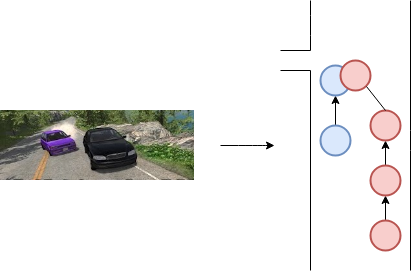
\includegraphics[scale= 0.4]{pictures/SO1_Beam_Net.png}
  \caption{Trajectory Network From BeamNG}
\end{figure}

In addition, the damage of the ego vehicle and the leading vehicle will be considered to know the exact point of impact on the roads and which region of the car is damaged. It will help us to separate critical (collision of cars) and non-critical (no collision of cars) scenarios in the large parameter space. Moreover, the numerical values will be monitored at every 0.5 sec to 1 sec to reduced the computation times and reduced the number of nodes on the graph. The NetworkX \cite{SciPyProceedings_11} library enable us to convert the continuous data into discrete nodes.     

\subsubsection{Simulation Categorization and Similarity Computation}
For the analysis of precrash and aftermath of car crash to calculate the accuracy of the simulation between the original simulation and predicted simulation. Both the critical and non-critical scenarios will be evaluated to choose the next parameter for the simulation.\\
Insert Image
The aftermath of car crash like striking car and victim car distance from the point of crash and deflection from the original path will be considered for both predicted and original network of nodes (Trajectory). Furthermore, the area or region of damage on the car with severity level required examination to compare with the original description. \\  


\begin{figure}[H]
\centering
  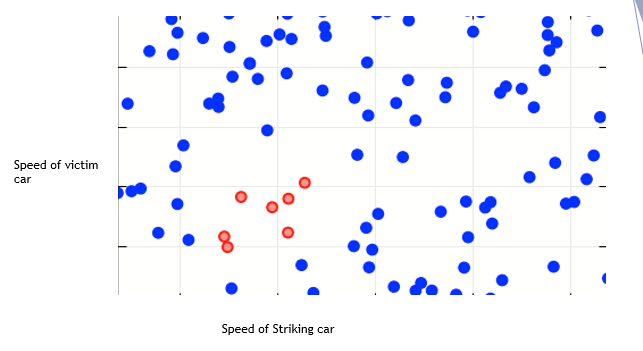
\includegraphics[scale = 0.4]{pictures/criticalandnoncriticalscenarios.png}
  \caption{Critical and Non Critical Scenarios}
\end{figure}


The primary focus of my research is to focus on the velocity and steering angle parameters of the car crash and analyze the behaviours of the self-driving car after the car crash. These parameters are usually are not described in the accident scenario and aid the autonomous vehicles in speed adjustment and safety of the car. Hence, i have to run a lot of simulations and categorize the critical scenarios and measure the distance and rotation quantities at each simulation. The top-K simulations will be selected to evaluate the end result of each simulation. 

The observable variables are Critical or Non Critical Scenario, Velocity,	Steering Angle,	Distance of striking car after impact, Rotation of car after impact.


\subsubsection{Parameters Tuning}
The selection of the next parameter in Test Case depend upon the search space and the accuracy of the reconstructed simulation of the test case. We can restrict the regions of the search space based on the feedback from the simulation and reduce the time of simulation and computation cost. Since, our evaluation is dependent upon the matching of frames of each simulation and choosing the best test case of the simulation from the Decision tree/ Binary Search Tree. For Example,In the initial scenario the ego car crash with the leading car with a speed/velocity of 20m/s and stays in the exact same position. However we have to explore the velocity at which the ego car crash with the leading car and go away from the impact point in the given direction. It means that we have to collide car with more momentum and speed to reproduce the desired scenario.